\documentclass[11pt]{memoireuqamV2}

%%%%%%%%%%%%%%%%%%%%%%%%%%%%%%%%%%%
% OVERLEAF: Utiliser TexLive 2021 %
%%%%%%%%%%%%%%%%%%%%%%%%%%%%%%%%%%%

% \usepackage{natbib}  % optionnel, doit être chargé avant babel
% \renewcommand{\cite}[1]{\citep{#1}}  % redéfinition utile

\usepackage[french]{babel}
\usepackage[utf8x]{inputenc} % Pour utiliser les caractères accentués
\usepackage[T1]{fontenc}
\usepackage{url}
\usepackage[a-1b]{pdfx}
\usepackage{hyperref}
\usepackage{lipsum}
\usepackage{layout}
\makeatletter
\renewcommand*{\lay@value}[2]{%
  \strip@pt\dimexpr0.351459\dimexpr\csname#2\endcsname\relax\relax mm%
}
\makeatother

% optionnel
\usepackage{graphicx}% Pour les figures
\usepackage{amsfonts}
\usepackage{standalone}
\usepackage{tikz}
\usepackage{pgfplots}

% police similaire à calibri, optionnelle (voir https://guidemt.uqam.ca/gabarit-et-mise-en-page/#ressource-697)
\usepackage[sfdefault,lf]{carlito}
% \usepackage{times}


%%%%%%%%%%%%
% Acronymes et symboles
%%%%%%%%%%%%
\usepackage[toc,acronym]{glossaries}
\defglsentryfmt[main]{\textbf{\glsgenentryfmt}}
\newglossary[slg]{symbols}{syi}{syg}{Notation}
\newglossary[def]{definitions}{syi}{syg}{Glossaire}
\loadglsentries{glossaires/notation}
\loadglsentries{glossaires/acronymes}
\loadglsentries{glossaires/glossaire}
\makenoidxglossaries

\begin{document}%\layout

%%%%%%%%%%%%%%%%%%%%
% Pour la page titre
%%%%%%%%%%%%%%%%%%%%
\title{Outils de classification taxonomique basés sur des réseaux neuronaux pour analyse de données métagénomiques}
% Votre nom complet tel qu'il apparaît à votre dossier du registrariat de l'UQAM
\author{Vincent Therrien}
% Année et mois courant sauf si spécifié autrement pas \degreemonth et \degreeyear
%\degreemonth{mois du dépôt}
%\degreeyear{année du dépôt}
\uqammemoire %% ou \uqamthese ou \uqamrapport ou \uqamprop
\matiere{informatique}


\pagenumbering{roman} % numérotation des pages en chiffres romains
\thispagestyle{empty}        % La page titre n'est pas numérotée
\maketitle
\stepcounter{page}

%%%%%%%%%%%%%%%%%%%%
% Page préliminaires
%%%%%%%%%%%%%%%%%%%%

\chapter*{Remerciements}
Je tiens à remercier Monsieur Vladimir Makarenkov pour ses précieux conseils et son accompagnement tout au long du projet ainsi que Madame Virginie Calderon pour m'avoir fait découvrir la richesse de la bioinformatique.

\tableofcontents % Pour générer la table des matières
\listoffigures% Pour générer la liste des figures
\listoftables % Pour générer la liste des tableaux

% Ici, on suppose une liste d'acronymes et une fiche de notation. Supprimez ces lignes si elles sont sans objet.
\glsaddall[types={acronym}]
\printnoidxglossary[type=acronym,toctitle=ACRONYMES,nonumberlist,sort=def]
\glsaddall[types={symbols}]
\printnoidxglossary[type=symbols,style=tree,nonumberlist,sort=def,toctitle=NOTATION]

\glsaddall[types={definitions}]
\printnoidxglossary[type=definitions,nonumberlist,sort=def,toctitle=GLOSSAIRE]

\glsresetall

\begin{abstract}
Le séquençage d'ADN rapide rend possible de nouvelles applications en biologie et en médecine.
Néanmoins, l'analyse d'un volume de plus en plus grand de données génomiques requiert des ressources
informatiques et un temps de calcul massifs, d'où l'importance de développer des outils d'analyse
efficaces.

La métagénomique étudie le matériel génétique prélevé dans les microbiomes, des communautés de
microorganismes qui vivent dans des habitats très variés comme le sol, l'eau, le système digestif
humain et d'autres environnements. Une meilleure compréhension des microbiomes est nécessaire pour
améliorer notre capacité à les caractériser, ce qui aiderait à détecter les pathogènes plus
efficacement ou mieux caractériser les sols en agriculture, par exemple. Une méthode répandue pour
analyser des métagénomes consiste à comparer des séquences d'ADN prélevées dans un environnement
avec des bases de données contenant des génomes de référence. Cette approche est toutefois lente et
limitée par la qualité des bases de données. Une technique plus récente et plus flexible consiste à
entraîner des réseaux neuronaux pour identifier les espèces présentes dans un métagénome, mais elle
requiert un temps d'entraînement important et comporte des difficultés en lien avec l'interprétation
des résultats.

Ce mémoire présente de nouvelles techniques de classification taxonomique des séquences d'ADN
métagénomique, ce qui consiste à catégoriser les organismes dans des groupes génétiquement
apparentés. Les techniques sont basées sur le modèle Mamba, un modèle à espace d'états, ainsi que
des variantes modifiées par un traitement parallèle en flux (Mamba-Dual), un pré-traitement par CNN
(Mamba-CNN), et une combinaison des deux améliorations (Mamba-Dual-CNN). Sur des ensembles de
séquences d'ADN génétiquement diversifiées, Mamba-Dual-CNN classifie les données avec une précision
moyenne de $89,97\%$, ce qui se compare favorablement à un transformateur de taille similaire
($72,46\%$), le modèle BERTax ($86,88\%$) et les outils MMSeqs 2 ($88,20\%$) ainsi que Kraken 2
($75,51\%$). La durée d'entraînement des modèles à espace d'états testés est outre moins longue
qu'un transformateur de taille similaire, avec $0,164\;s$ pour un pas avec Mamba-Dual-CNN contre
$0,188\;s$ pour le transformateur.

\end{abstract}

% Utilisez l'environnement  abstract pour rédiger votre résumé

%%%%%%%%%%%%%%%%%%%%
% Document principal
%%%%%%%%%%%%%%%%%%%%
\pagenumbering{arabic}

% Utilisez l'environnement  introduction pour rédiger votre introduction
\begin{introduction}
\label{chapitre:introduction}

Les technologies de séquençage d'ADN permettent aujourd'hui d'analyser de grandes quantités de
matériel génétique. Alors que la première génération de technique de séquençage (à partir des années
1970) était limitée à un faible débit, les technologies de deuxième génération (aussi appelées
<<nouvelle génération>> ou \textit{NGS}, à partir des années 2000) ont grandement augmenté la
vitesse de séquençage mais demeuraient limitées à de courtes séquences d'au plus quelques centaines
de nucléotides. Les technologies de troisième génération (à partir des années 2010) constituent une
autre amélioration qui permet d'analyser des séquences encore plus longues, jusqu'à plusieurs
milliers de nucléotides, encore plus rapidement \cite{satam2023}. Ces technologies ont contribué à
améliorer nos connaissances en génomique et mené à des applications en biologie et médecine, par
exemple, pour la détection de pathogènes, les diagnostics cliniques, la protection de
l'environnement et l'agriculture \cite{liu2025}. De nombreux outils ont aussi été développés pour
analyser les données de séquençage et faciliter le travail des chercheurs \cite{roy2024}. Ce mémoire
s'intéresse en particulier à une application de l'analyse de séquences d'ADN, la classification
taxonomique de métagénomes, qui vise à identifier les espèces présentes dans des microbiomes.

La métagénomique se heurte à des problèmes majeurs. Le \textbf{volume de données} complique les
analyses. Un séquençage conventionnel de métagénome avec des technologies de troisième génération
peut générer $10\;Go$ de données par expérience \cite{PerezCobas2020}. Les bases de données
contiennent aussi beaucoup d'information : RefSeq \cite{refseq} contient des génomes de référence de
haute qualité pour plus de $176\;395$ organismes en avril 2026 et GTDB \cite{gtdb} contient un
taxonomie exhaustive pour plus de $153\;000$ espèces de procaryotes. Identifier une espèce en
comparant une séquence d'ADN avec une base de données de référence entraînerait un temps de calcul
inacceptable pour des applications réelles, c'est pourquoi de nombreuses méthodes d'analyse ont été
développées pour obtenir des résultats plus rapidement \cite{roy2024}. La \textbf{fiabilité des
résultats} fait référence à la confiance qu'on peut accorder aux données produites par une analyse
métagénomique. Gihawi et al expliquent qu'une étude métagénomique influente était basée sur une
analyse erronée : en normalisant mal les données et en utilisant des séquences contaminées par l'ADN
humain, les chercheurs de cette étude en étaient venus à la conclusion qu'il est possible de prédire
certains types de cancers à partir de données de microbiotes humains, ce qui a induit d'autres
chercheurs en erreur \cite{gihawi2023}. Il est donc impératif de développer des techniques d'analyse
qui soient non seulement efficaces, mais aussi rigoureuses et facile à interpréter pour éviter
d'autres scénarios du même genre.

Ce mémoire vise à améliorer des techniques de classification taxonomique de données de séquençage
métagénomique, ce qui implique les étapes principales suivantes :

La \textbf{génération de données synthétiques} permet de créer des ensembles de données pour
entraîner et valider les outils de classification. Les données doivent être générées à partir de
séquences de haute qualité et représenter des échantillons métagénomiques variés pour éviter de
surajuster les modèles et d'obtenir des performances non représentatives d'un cas d'utilisation
réel.

L'élaboration de \textbf{modèles de classification taxonomique} consiste à concevoir des réseaux
neuronaux inédits pour améliorer les techniques existantes. Ces modèles doivent offrir des
performances supérieures en terme d'utilisation de ressources informatiques (temps de calcul et
utilisation de la mémoire) et de classification (précision plus élevée).

L'\textbf{entraînement des modèles} consiste à modifier automatiquement les paramètres des modèles
pour leur permettre d'effectuer les classifications taxonomiques. Cette étape requiert des
ressources intensive et doit s'appuyer sur de bons hyperparamètres pour converger vers une solution
efficace. Un entraînement mal configuré peut faire échouer le modèle à apprendre comment résoudre
une tâche et ainsi causer un gaspillage de ressources \cite{liu-etal-2020-understanding}.

Ce projet consiste à répertorier des architectures de réseaux neuronaux utilisés en métagénomique et
encore non appliqués à la métagénomique qui ont le potentiel d'offrir de meilleures performances.
Après la sélection des modèles, le processus d'entraînement est ajusté pour chaque modèle afin de
maximiser leurs performances. Les hyperparamètres sont modifiés et différentes techniques
d'entraînement sont testées pour déterminer les meilleures manières d'obtenir une classification de
haute qualité. Tous les modèles sont ensuite testés avec les mêmes données de test et d'entraînement
pour identifier les modèles les plus efficaces. On compare aussi les nouveaux modèles développés
dans le cadre de ce projet avec des techniques de classification développées par d'autres équipes de
chercheurs pour confirmer que les nouveaux modèles constituent bel et bien des amélioration par
rapport aux outils déjà existants.

Ce mémoire présente les contributions principales suivantes :

\begin{list}{$\bullet$}{}
    \item Comparaison systématique de différentes architectures de réseaux neuronaux pour la
        classification taxonomique de données métagénomique, en particulier une comparaison
        approfondie entre les transformateurs et les modèles à espace d'état (SSM).
    \item Étude des effets du pré-entraînement et de l'ajustement sur les performances des modèles
        de classification.
    \item Étude des effets du prétraitement des données de séquençage (jetonisation et traitement
        par CNN) sur les performances des modèles de classification.
    \item Conception de modèles de réseaux neuronaux inédits spécifiquement développés pour la
        classification taxonomique.
    \item Analyse de la consommation de ressources informatique par les modèles d'AA.
    \item Publication du code source ouvert pour répliquer tous les résultats du projet.
\end{list}

Ce mémoire comporte quatre sections principales. Le chapitre 1 présente un état de l'art des outils
d'analyse de données métagénomique ainsi que de l'apprentissage profond, avec un accent particulier
sur les réseaux neuronaux dédiés aux analyses de données génomiques. Le chapitre 2 explique la
méthodologie du projet : collecte et transformation des données, conception des modèles,
entraînement et évaluation. Le chapitre 3 présente les résultats des modèles. Le chapitre 4 discute
des résultats et propose des améliorations possibles aux nouveaux modèles.

\end{introduction}

\chapter{État de l'art}
\label{chapitre:1}
Ce chapitre présente une revue de littérature sur les sujets en lien avec la classification
taxonomique de données métagénomiques. Elle discute des technologies de séquençage, bases de
données, techniques d'analyses classiques et techniques basées sur l'apprentissage automatique

\section{Séquençage d'ADN}
Les technologies de séquençage servent à obtenir des séquences de
caractères qui indiquent la structure de molécules d'ADN or d'ARN. Le tableau
\ref{tableau:techniques_de_sequencage} présente quelques technologies de
séquençage d'ADN \cite{satam2023}.

\begin{table}[hbt!]
    \centering
    \begin{tabular}{lp{0.16\linewidth}p{0.13\linewidth}p{0.42\linewidth}}
\hline
Nom de la technologie & Principe de séquençage & Longueur des séquences & Limites \\
\hline
454 pyrosequencing & Synthèse & $400$ à $1000$ & Peut contenir des erreurs de délétion et insertion \\
Ion Torrent & Synthèse & $200$ à $300$ & Perte de signal lors du séquençage d'homopolymères \\
Illumina & Synthèse & $36$ à $300$ & Taux d'erreur de séquençage jusqu'à $1\%$ dans certains cas. \\
SOLiD & Ligation & $75$ & Erreurs de substitution et sous-représentation des régions riches en GC \\
PacBio SMRT & Synthèse & $10k$ à $25k$ & Coût élevé comparé aux autres méthodes \\
Oxford Nanopore & Détection d'impédance & $10k$ à $30k$ & Taux d'erreur de séquençage jusqu'à $15\%$ dans certains cas. \\
\hline
    \end{tabular}
    \caption{Survol de technologies de séquençage d'ADN}
    \label{tableau:techniques_de_sequencage}
\end{table}

Il est nécessaire de suivre un protocole expérimental pour séquencer correctement
du matériel génétique. Navguire et al \cite{Navgire2022} présentent les étapes
fondamentales suivantes d'un tel protocole :

\begin{enumerate}
    \item \textbf{Collecte d'échantillon} : Le matériel génétique est prélevé
        dans un environnement à un instant donné et sous des conditions
        spécifiques. Par exemple, le métagénome de la rhizosphère d'une plante
        peut être échantillonné à une étape précise de son développement et le
        microbiome fécal humain peut être échantillonné un temps défini après
        l'administration d'un vaccin à un patient.
    \item \textbf{Isolation de l'ADN} : L'échantillon est traité en vue du
        séquençage, par exemple, en ajoutant des réactifs pour provoquer la
        lyse des cellules et libérer leur matériel génétique. Le processus exact
        d'isolation de l'ADN dépend du type d'échantillon et doit préserver le
        maximum de diversité dans l'échantillon pour éviter de déformer l'abondance
        de certains organismes.
    \item \textbf{Préparation de la bibliothèque} : L'ADN isolé est adapté à
        une technologie de séquençage particulière, ce qui mène à la création
        d'une bibliothèque de fragments d'ADN. À la fin de cette étapes, les
        fragments d'ADN ont des longueurs similaires et comprennent des adapteurs
        connus aux extrémités $5'$ et $3'$.
    \item \textbf{Séquençage} : La bibliothèque est traitée par une technologie
        de séquençage, qui génère des fichiers contenant les lectures des
        fragments d'ADN. Les données de lecture peuvent ensuite être utilisées
        pour réaliser une analyse de la composition de l'échantillon. Le
        séquençage peut prendre quelques minutes pour de petites bibliothèques
        avec certaines technologies de séquençage comme Oxford Nanopore mais
        prend généralement plusieurs heures, voire plusieurs jours \cite{roy2024}.
\end{enumerate}

Il existe deux approches principales pour l 'étape 3 (préparation de la bibliothèque). Dans le cadre
d'une analyse métagénomique \textbf{basée sur les gènes marqueurs} (\textit{marker-gene
metagenomics}), des régions spécifiques des métagénomes sont amplifiées et séquencées. Ces régions
sont sélectionnées en fonction de leur capacité à identifier des espèces spécifiques. Par exemple,
les gènes d'ARN ribosomique 16S ont tendance à être conservés au cours de l'évolution et peuvent
être utilisés pour identifier des espèces de bactéries. Toutefois, puisque les gènes peuvent être
transférés entre certains organismes et que les gènes marqueurs sont relativement courts, cette
approche, bien que peu dispendieuse, est limitée à une faible sensitivité \cite{Matchado2024}. Une
variante de cette approche consiste à utiliser des séquences plus longues que les gènes marqueurs
seuls, ce qui peut améliorer les performances \cite{BenitezPaez2022}. La seconde approche de
préparation d'une bibliothèque est le \textbf{séquençage complet du génome} (\textit{whole genome
sequencing}), qui consiste à séquencer tous les fragments présents dans l'échantillon. Cette
approche est plus dispendieuse parce qu'elle requiert le séquençage d'un volume beaucoup plus grand
de matériel génétique, mais elle permet des analyses métagénomiques plus poussées parce que
davantage de données sont disponibles. Un désavantage de cette approche est sa sensibilité à l'ADN
dominant dans un échantillon; par exemple, dans un échantillon de microbiome humain, l'ADN humain
peut être surreprésenté et rendre l'ADN microbien plus difficile à analyser \cite{Matchado2024}. Ce
phénomène est moins susceptible de survenir dans les analyses basées sur les gènes marqueurs parce
que l'ADN humain ne comprend pas les séquences cibles.

\section{Bases de données}
La communauté scientifique maintient des bases de données publiques afin de faciliter la réplication
de leurs études et d'améliorer l'état des connaissances en biologie. Cette section en présente
quelques-unes qui sont pertinentes pour la classification taxonomique.

\subsection{Bases de données de séquençage}
Les bases de données de séquençage contiennent des séquences biologiques (protéines ou nucléotides)
qui décrivent des génomes complets ou simplement des sections de génomes.

\begin{list}{$\bullet$}{}
    \item GenBank \cite{genbank} est une base de données ouverte de toutes les séquences de
        nucléotides publiquement disponibles ainsi que leurs traduction en protéine, produite et
        maintenue par le NCBI. En 2024, GenBank comprenait plus de $4,7$ milliards de séquences de
        nucléotides appartenant à plus de $580\;000$ espèces.
    \item RefSeq \cite{refseq} est une base de données ouverte de séquences de nucléotides et
        protéines publiquement disponibles, produite et maintenue par le NCBI. Contrairement à
        GenBank, RefSeq contient une seule séquence de référence pour chaque molécule biologique et
        les séquences de RefSeq sont annotées pour leur assigner des informations supplémentaires,
        comme les fonctions biologiques des séquences. Les séquences de RefSeq sont ainsi moins
        redondantes et plus fiables que celle de GenBank, mais aussi moins nombreuses. Les données
        de RefSeq sont enregistrées uniquement pour $176\;395$ organismes en mars 2026.
    \item Ensembl \cite{ensembl} est un projet qui se concentre principalement sur l'annotation de
        génomes de vertébrés. Au lieu d'effectuer des annotations sur des séquences biologiques
        comme RefSeq, Ensembl les effectue plutôt à même des génomes d'organismes. La base de
        données contient les génomes de $4700$ espèces en mars 2026.
\end{list}

\subsection{Bases de données taxonomiques}
Les bases de données taxonomiques décrivent les liens entre des organismes, ce qui permet d'assigner
des organismes à des groupes particuliers.

\begin{list}{$\bullet$}{}
    \item NCBI Taxonomy \cite{ncbi_tax} est une base de données taxonomique maintenue par le NCBI.
        Elle classifie hiérarchiquement tous les organismes ayant au moins une séquence enregistrée
        dans une base de données du INSDC, qui comprend GenBank. NCBI Taxonomy ne constitue pas un
        arbre phylogénétique; il est plutôt un outil de classification taxonomique qui aide à
        organiser les espèces mais ne représente pas exactement leurs liens évolutifs. Par
        conséquent, certaines séquences ne sont pas attribuées à des n\oe uds particuliers dans
        la hiérarchie taxonomique, ce qui rend leurs relations avec les autres espèces peu claire.
        Aussi, la base de données est régulièrement mise à jour, ce qui peut entraîner des problèmes
        de compatibilité de version entre certains outils.
    \item GTDB \cite{gtdb} est une base de données phylogénétique moderne pour les bactérie et
        archées maintenue par le Australian Centre for Ecogenomics et l'Université de Queensland.
        GTDB normalise les rangs taxonomiques par distance évolutive, ce qui signifie que des taxons
        d'un même niveau taxonomique comprennent une diversité génétique similaire. Cette
        caractéristique est bénéfique pour les outils de classification parce que la base de données
        comprend moins d'anomalies que NCBI Taxonomy. Toutefois, GTDB est limité à deux domaines du
        vivant et ne contient aucune information sur les eucaryotes et les virus.
\end{list}

\section{Analyse des séquences}
Les analyses métagénomiques se divisent en deux principaux types : les analyses taxonomiques et
les analyses fonctionnelles.

\subsection{Analyses taxonomiques}
Les analyses taxonomiques consistent à comparer les lectures d'ADN à des bases de données de
référence pour identifier les organismes présents dans un échantillon \cite{Navgire2022}. Plus
particulièrement, le profilage vise à estimer l'abondance relative des organismes présents dans un
échantillon et la classification, à identifier le plus précisément possible les espèces présentes
dans un échantillon. La classification peut être effectuée avec des lectures ou encore avec des
contigs élaborées à partir des lectures brutes. En général, les analyses taxonomiques s'appuient
généralement sur les séquences d'ADN seules et n'utilisent pas d'annotations fonctionnelles. Les
analyses taxonomiques peuvent s'appuyer sur plusieurs outils.

\subsubsection{Kraken2}
Kraken \cite{kraken} est une suite d'outils de classification, quantification et visualisation
métagénomique. La suite inclut quatre versions du logiciel :

\begin{list}{$\bullet$}{}
    \item \textbf{Kraken} classifie les lectures d'ADN à partir d'une base de données de K-mers en
        prenant, en général, $K = 31$. Les K-mers de l'échantillon sont comparés à la base de
        données pour identifier des correspondances exactes et déterminer le cénancêtre des génomes
        qui contiennent les mêmes K-mers. L'avantage de cet algorithme est que même si une espèce
        présente dans l'échantillon n'est pas représentée dans la base de donnée, il est possible
        de lui assigner groupe taxonomique plus général (ex. la famille au lieu du genre) \cite{kraken1}.
        Néanmoins, comme Kraken emmagasine des K-mers entier, il requiert beaucoup de mémoire et
        offre de faibles performances \cite{kraken}.
    \item \textbf{KrakenUniq} est une variante de Kraken qui distingue (1) les correspondances entre
        les lectures de l'échantillon avec la base de données et (2) les correspondances uniques de
        K-mers. Cela lui permet de consider la couverture de plusieurs régions différentes des
        génomes de référence et évite les biais en faveur des régions hautement conservées, mais
        augmente la quantité de mémoire à utiliser \cite{kraken}.
    \item \textbf{Kraken 2} modifie l'algorithme original de Kraken pour utiliser une correspondance
        statistique entre les lectures et la base de données au lieu de correspondances exactes, ce
        qui entraîne deux bénéfices : (1) Kraken 2 emmagasine un sous-ensemble de K-mers, ce qui
        diminue la taille de la base de données de $85\%$, et (2) Kraken 2 est plus résilient aux
        erreurs de séquençages et aux indels. Cette variante est recommandée pour les analyses de
        microbiome \cite{kraken}.
    \item \textbf{Kraken2Uniq} combine les correspondances statistiques de Kraken 2 et le traçage
        de régions distinctes de KrakenUniq. Cette variante est recommandée pour l'identification de
        pathogènes parce qu'elle s'avère plus sensible à des espèces précises mais requiert des
        ressources informatiques plus grandes \cite{kraken}.
\end{list}

La suite logicielle Kraken contient par ailleurs KrakenTools et Pavian, des outils d'analyse
statistique et de visualisation des résultats. Des outils tiers sont généralement requis pour
réaliser une analyse complète. Par exemple, avec de courtes lectures d'ADN produites par des
appareils de la plateforme Illumina ($100$ à $250$ nucléotide par lecture), il est d'abord
nécessaire de former des contigs avec un logiciel comme Bowtie \cite{kraken}.

\subsubsection{bracken}
Bracken \cite{bracken} est un logiciel de profilage taxonomique basé sur Kraken.
Kraken n'est pas conçu pour mesurer les abondances relatives de groupes taxonomiques présents dans
un échantillon; il sert plutôt à identifier des espèces précises. Comme plusieurs séquences d'ADN
sont communes à plusieurs espèces à cause de régions hautement conservées ou de transferts
horizontaux, Kraken assigne aux lectures correspondantes des taxons génériques, ce qui rend les
résultats impropres à une analyse d'abondance. Bracken modifie les résultats de Kraken en
redistribuant les lectures à travers un arbre phylogénétique par une méthode probabiliste, ce qui
les rend apte à une analyse d'abondances.

\subsubsection{MetaPhlAn 3}
MetaPhlAn 3 \cite{metaphlan3} est un logiciel de classification taxonomique qui utilise une approche
basée sur les gènes spécifiques à des clades, c'est-à-dire des gènes qui se trouvent universellement
dans un groupe taxonomique donné et qui sont universellement absents à l'extérieur de ce groupe. Au
lieu d'indexer des génomes entiers, MetaPhlAn 3 aligne uniquement les gènes marqueurs avec une base
de données de référence d'environ $1,1$ millions de gènes en utilisant Bowtie. Cette approche permet
d'assigner avec une grande précision les lectures contenant des gènes marqueurs à un groupe
taxonomique, mais les lectures ne comprenant pas de tels gènes (la majorité des lectures, dans la
plupart des cas) ne peuvent pas être assigné à un taxon.

\subsubsection{mOTUs3}
mOTUs3 \cite{motus} est un logiciel de classification taxonomique qui utilise des gènes marqueurs
métagénomiques. Ces marqueurs sont définis d'une manière similaire à la base de données utilisée par
MetaPhlAn 3, mais au lieu d'être générés exclusivement à partir de génomes de référence, ils sont
aussi générés à partir de métagénomes assemblés. Cela permet à mOTUs3 de regrouper des lectures dans
des groupes taxonomiques qui n'ont pas de génome de référence officiel (dans un tel cas, Kraken 2
leur assigne un groupe taxonomique plus élevé et MetaPhlAn 3 ne peut pas faire de classification).

\subsubsection{sourmash}
Sourmash \cite{sourmash} est un logiciel de profilage taxonomique qui estime les abondances de
groupes taxonomiques en comparant des jeux de données compressés. Le logiciel est basé sur
l'algorithme de compression avec pertes FracMinHash, qui préserve un sous-ensemble restreint des
K-mers présents dans les lectures d'ADN nommé signature. Des signatures peuvent être comparées par
similarité de Jaccard sans effectuer de comparaisons intensives des séquences afin d'estimer les
compositions taxonomiques d'échantillons.

\subsubsection{Centrifuge}
Centrifuge \cite{centrifuge} est un logiciel de classification taxonomique qui utilise la
transformation de Burrows-Wheeler pour créer une base de données optimisée pour la recherche de
séquences et l'indice de Ferragina-Manzini pour optimiser la recherche. Au lieu d'effectuer des
correspondances avec des K-mers d'une longueur prédéfinie comme Kraken 2, Centrifuge recherche les
correspondances les plus longues possibles entre les lectures séquencées et la base de données de
référence.

\subsubsection{MetaMaps}
MetaMaps \cite{metamaps} est un logiciel de classification taxonomique spécialisé pour les longues
séquences. Il fonctionne en deux étapes. MetaMaps utilise d'abord un algorithme de mappage basé sur
la minimisation pour approximer les endroits dans une base de données de référence où les lectures
pourraient avoir des correspondances. Ensuite, il utilise un algorithme d'espérance-maximisation
pour évaluer la qualité des correspondances potentielles et identifier les taxons d'où proviennent
les lectures.

\subsubsection{MMSeqs2}
MMSeqs2 \cite{mmseqs2} est une suite logicielle conçue pour la recherche et le groupement rapide
dans les bases de données de protéines et de nucléotides. Il utilise trois étapes pour effectuer des
alignements efficacement : (1) pré-filtrage des correspondances potentielles par K-mers, (2)
alignements sans indels et (3) alignement avec indels de Smith-Waterman. Le module MMSeqs2 Taxonomy
permet d'effectuer des classifications taxonomiques en traduisant les lectures d'ADN selon les six
cadres de lecture et en comparant des séquences d'acides aminés. Cette approche permet de
reconnaître des liens évolutifs entre des séquences qui ont divergé au niveau des séquences de
nucléotides mais qui ont conservé la même structure de protéine, ce qui constitue un avantage qui
n'est pas accessible aux techniques précédemment présentées.

\subsubsection{BugSeq}
BugSeq \cite{bugseq} est un logiciel de classification taxonomique spécialisé pour les lectures
nanopores (c-à-d longues séquences). Il combine des outils d'alignement de lectures et de recherche
de cénancêtre basé sur un processus bayésien. Contrairement aux autres outils, qui sont livrés
comme des programmes autonomes, BugSeq est un pipeline qui cascade plusieurs logiciels.

\subsubsection{MEGAN et MEGAN-LR}
MEGAN et MEGAN-RL \cite{meganlr} sont des logiciels d'analyse de métagénome respectivement conçus
pour les analyses des lectures courtes et longues. Un peu comme MMSeqs2, ces outils sont basés sur
une analyse de séquences de protéines traduites à partir des cadres de lecture des séquences de
nucléotides. Un aspect important de MEGAN est sa capacité à corriger les décalage dans les cadres
de lecture pour permettre de corriger les séquences de protéines malgré les indels.

\subsection{Analyses fonctionnelles}
Les analyses fonctionnelles consistent à étudier des fonctions particulières, comme les gènes de
résistance aux antimicrobiens \cite{Navgire2022}. Elles se divisent en deux étapes. La prédiction de
gènes sert à déterminer quelles séquences d'ADN correspondent à un gène d'intérêt et l'annotation
fonctionnelle, à y assigner une fonction particulière. Les analyses fonctionnelles s'appuient sur
les séquences mais aussi sur des bases de données qui décrivent les fonctions de gènes. Comme ce
mémoire se concentre sur les techniques de classification taxonomique, ces techniques sont ici
présentées brièvement.

\begin{list}{$\bullet$}{}
    \item BLAST \cite{blast} est un logiciel qui trouve des régions de similarité entre des
        séquences de protéines ou de nucléotides grâce à la minimisation basée sur les K-mers. Il
        s'agit d'un outil plus ancien et moins efficace que MMSeqs2, mais il demeure largement
        utilisé, entre autre grâce à son intégration au serveur du NCBI qui permet d'effectuer des
        requête contre des bases de données.
    \item DIAMOND \cite{diamond} est un logiciel d'alignement adapté aux données métagénomiques qui
        rapporte un temps d'exécution jusqu'à $20\;000$ fois plus rapide que BLAST pour les
        séquences courtes avec un degré de sensibilité similaire à BLAST. Au lieu d'utiliser des
        K-mers, DIAMOND utilise un double indice, c'est-à-dire que la séquence recherchée ainsi que
        la base de données sont indexées pour faciliter la recherche de correspondances. DIAMOND est
        aussi plus résilient aux mutations que BLAST parce qu'il ne recherche pas de correspondances
        parfaites entre les séquences.
\end{list}

\section{Apprentissage automatique}
L'apprentissage automatique \cite{oqlfAA} consiste à permettre à un ordinateur d'apprendre à
résoudre un problème sans spécifier explicitement de méthodes de résolution \cite{samue1959}, par
exemple, en laissant un algorithme de classification d'image améliorer sa précision sans
interventions manuelles. Il s'agit d'un domaine vaste de recherche; cette section en présente
seulement les principes de bases, les architectures de réseaux neuronaux les plus utilisées et leur
application à la métagénomique.

\subsection{Principes de base de l'apprentissage automatique}
L'apprentissage automatique se divise en quatre principaux types.

\subsubsection{Apprentissage supervisé}
L'apprentissage supervisé consiste à entraîner des modèles en leur fournissant des données
étiquetées, c'est-à-dire des données pour lesquelles une valeur cible est connue. Suivant la
notation employée par \cite{vapnik1995}, on définit :

\begin{equation}
    \begin{cases}
        X = \{x_1, x_2, x_3, ... \}, x_i \in R^n, \text{Un ensemble de vecteurs à classifier} \\
        Y = \{y_1, y_2, y_3, ... \}, \text{Valeurs cibles pour chaque vecteur à classifier} \\
        \alpha, \text{Un ensemble de paramètres à déterminer} \\
        f(x, \alpha), \text{Une fonction qui cherche à prédire $y_i$} \\
        \hat{Y} = \{\hat{y}_1, \hat{y}_2, \hat{y}_3, ... \}, \text{Valeurs prédites par $f(x, \alpha)$ pour chaque $x_i$}
    \end{cases}
\end{equation}

On suppose que les valeurs cibles sont tirées d'une distribution inconnue $F(y_i | x_i)$. On mesure
l'écart entre une valeur cible attendue, $y$, et une valeur cible prédite, $f(x, \alpha)$, au moyen
d'une fonction de perte $L(y, f(x, \alpha))$. Afin de choisir les meilleurs paramètres pour
approximer au mieux la distribution $F(y_i | x_i)$, on doit minimiser l'équation \ref{eq:risque}.

\begin{equation}
    \label{eq:risque}
    \begin{split}
        R(\alpha) &= \int L(y, f(x, \alpha)) dF(x, y) \\
                  &= \frac{1}{k} \sum_{i=1}^{k} L(y_i, f(x_i, \alpha)) \;\;\; \text{(pour des valeurs discrètes)}
    \end{split}
\end{equation}

Par conséquent, les paramètres optimaux $\alpha^*$ sont obtenus par l'équation \ref{eq:minim_risque}.

\begin{equation}
    \label{eq:minim_risque}
    \alpha^* = \arg \min_{\alpha} \frac{1}{k} \sum_{i=1}^{k} L(y_i, f(x_i, \alpha))
\end{equation}

L'apprentissage supervisé vise principalement les problèmes de classification et de régression, pour
lesquelles les valeurs de $Y$ sont respectivement discrète ou continues. Cette approche est
particulièrement utilise en classification de données métagénomiques parce que les bases de données
annotées contiennent des séquences d'ADN appartenant à des taxons connus.

\subsubsection{Apprentissage non supervisé}
L'apprentissage supervisé consiste à entraîner des modèles en leur fournissant des données non
étiquetées, c'est-à-dire des données pour lesquelles aucune valeur cible n'est connue. Au lieu de
minimiser l'écart entre une prédiction et une cible, on cherche les paramètres $\alpha$ qui
modélisent les propriétés d'une distribution $F(x)$. Cette approche comprend plusieurs applications
\cite{hasti2009}; nous en présentons deux principales.

Le regroupement de données par classes (\textit{data clustering}) consiste à assigner à chaque
donnée $X = \{x_1, x_2, ..., x_n\}$ une classe $S = \{s_1, s_2, ..., s_k\}$ en minimisant la variance
intra-classe, donnée par l'équation \ref{eq:groupement}

\begin{equation}
    \label{eq:groupement}
    arg min_{S} \sum_{i=1}^{k} \sum_{x \in s_i} (x - \mu_i)^2,
\end{equation}

où $\mu_i$ désigne le centroïde des données dans la classe $s_i$.

La compression de données vise à minimiser l'erreur de reconstruction entre l'entrée $x$ et une
version $\hat{x}$ reconstruite après compression, tel qu'indiqué par l'équation
\ref{eq:compression}.

\begin{equation}
    \label{eq:compression}
    \alpha^* = arg min_{\alpha} \sum_{i = 1}^{n} \left[ x_i - g_\alpha (f_\alpha (x_i)) \right]^2
\end{equation}

L'apprentissage non supervisé permet d'extraire des propriétés de données non étiquetées, ce qui est
le cas pour les bases de données très volumineuses où l'étiquetage serait trop coûteux.

\subsubsection{Apprentissage semi-supervisé}
L'apprentissage semi-supervisé combine les approches supervisée et non supervisée pour entraîner des
modèles à partir de données étiquetées et non étiquetées, ce qui permet d'atteindre des performances
supérieures aux approches prises séparément et la rend intéressant pour la métagénomique, où des
bases de données complémentaires peuvent être utilisées. En général, cette approche minimise une
fonction qui comporte une perte supervisée et une perte de régulation non supervisée
\cite{chapelle2006}.

\subsubsection{Apprentissage auto-supervisé}
L'apprentissage auto-supervisé \cite{doersch2017} est une phase préparatoire de l'apprentissage
supervisé ou non supervisé qui consiste à entraîner un modèle à reconnaître les signaux les plus
utiles dans les données, ce qui permet d'augmenter les performances lors de la principale phase
d'entraînement.

\subsubsection{Apprentissage par renforcement}
L'apprentissage par renforcement \cite{sutton2018} diffère des autres approches parce qu'elle
consiste à laisser un modèle interagir dynamiquement avec un autre système. Cette approche est peu
fréquente dans la métagénomique parce que les analyses de séquences sont basées sur des données non
dynamiques.

\subsection{Réseaux neuronaux}
Les réseaux neuronaux, aussi appelés réseaux de neurones artificiels, sont une famille de
modèles d'apprentissage automatique basés sur des unités de traitement nommées neurones artificiels
inspirées des neurones biologiques \cite{goodfellow2016}.

\subsubsection{Entraînement}

L'équation \ref{eq:neurone} montre la modélisation mathématique d'un neurone artificiel.

\begin{equation}
    \label{eq:neurone}
    z = f \left( \sum_{i = 1}^{n} w_i x_i + b \right)
\end{equation}

où $z$ est la valeur de sortie du neurone, $x_i$ est une valeur d'entrée, $w_i$ est un paramètre
associé à une entrée nommée \textit{poids}, $b$ est un paramètre nommé \textit{biais} et $f(\cdot)$
est une fonction non linéaire nommée \textit{fonction d'activation}. Un réseau neuronal est composé
d'un ensemble de telles unités. La forme la plus simple est le perceptron multicouche, illustré par
la figure \ref{fig:pmc}.

\begin{figure}[h]
    \centering
    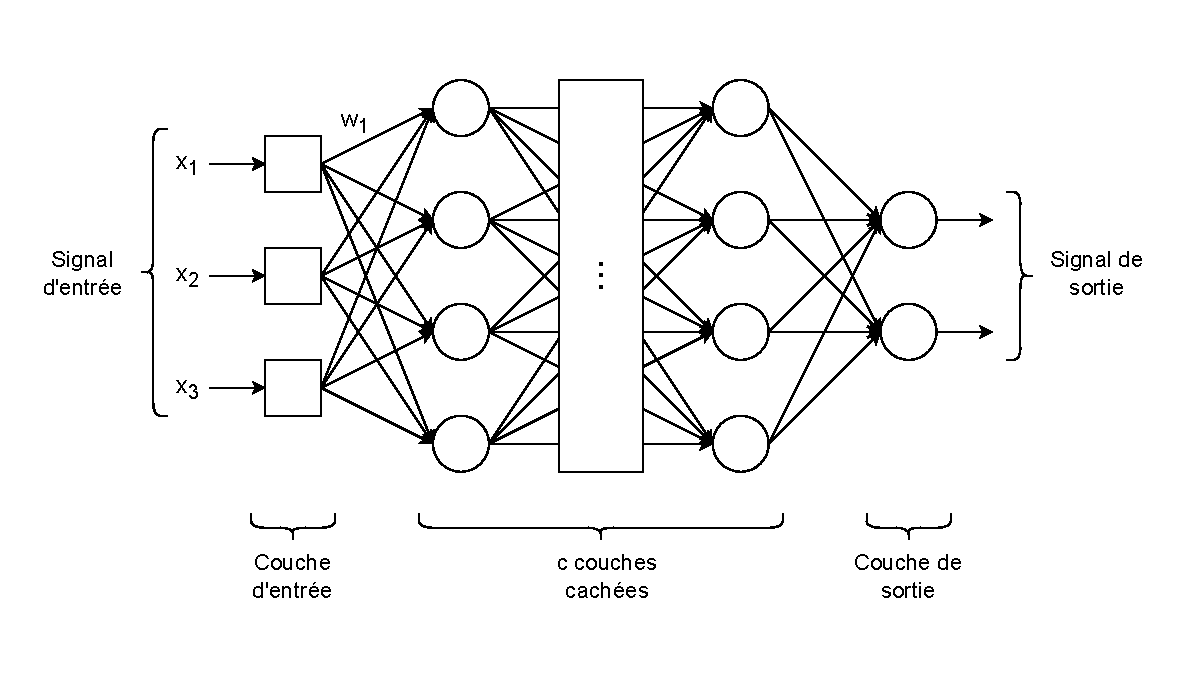
\includegraphics[width=0.9\linewidth]{figures/pmc.pdf}
    \caption{Diagramme d'un perceptron multicouche}
    \label{fig:pmc}
\end{figure}

Chaque cercle dans la figure \ref{fig:pmc} représente un neurone qui calcule l'équation
\ref{eq:neurone} en prenant $x_i$ comme une valeur transmise par la couche précédente (représentée
par une flèche), $w_i$ comme un paramètre ajustable associé à chaque entrée et $b$ comme un
paramètre ajustable distinct des entrées. Un réseau neuronal comportant plusieurs couches cachées
est dit \textit{profond} \cite{lecun2015}. La sortie $\mathbf{h}$ d'une couche de $n$ neurones
recevant un vecteur d'entrées $\mathbf{x}$ de $m$ valeurs est

\begin{equation}
    \label{eq:propagation_avant}
    \mathbf{h}_{n \times 1} = f \left( \mathbf{W}_{n \times m} \mathbf{x}_{m \times 1} + \mathbf{b}_{n \times 1} \right).
\end{equation}

L'équation \ref{eq:propagation_avant} calcule la propagation avant du réseau. On compare la sortie
finale du réseau avec un résultat cible $\mathbf{y}_{k \times 1}$ au moyen d'une fonction de coût
\ref{eq:cout} qui quantifie l'erreur du réseau.

\begin{equation}
    \label{eq:cout}
    C(y, \hat{y}) = \sum_{i=1}^{k} L(y_i, \hat{y})
\end{equation}

où $L( \cdot )$ est une fonction de perte, par exemple, $L(y_i, \hat{y}) = (y - \hat{y})^2$. La
rétropropagation consiste à calculer l'erreur associée à chaque neurone pour ajuster les paramètres
de façon à minimiser le coût. L'erreur $e_i^{(n)}$ du neurone $j$ de la couche $n$ est donnée par
l'équation \ref{eq:partiel}.

\begin{equation}
    \label{eq:partiel}
    e_i^{(n)} = \frac{\partial C}{\partial h_i^{(n)}}
\end{equation}

Par la règle de la dérivée en chaîne, on calcule l'erreur associée à un neurone d'une couche
précédente avec l'équation \ref{eq:retropropagation}.

\begin{equation}
    \label{eq:retropropagation}
    e_j^{(n - 1)} = f\prime^{(n - 1)} (h_j^{(n - 1)}) \sum_i w_{ij}^{(n)} e_i^{(n)}
\end{equation}

On propage l'erreur jusqu'à la couche initiale du réseau. Ce processus se nomme rétropropagation et
permet d'obtenir une erreur pour chaque neurone, laquelle sert à ajuster les paramètres par
l'équation \ref{eq:ajustement}.

\begin{equation}
    \label{eq:ajustement}
    \begin{split}
        w_{ij}^{(n)} &= w_{ij}^{(n)} - \lambda \cdot e_i^{(n)} x_i^{(n - 1)} \\
        b_i^{(n)} &= b_i^{(n)} - \lambda \cdot e_i^{(n)} \\
    \end{split}
\end{equation}

oè $\lambda \in [0, 1]$ est un taux d'apprentissage qui détermine la vitesse à laquelle les paramètres sont mis
à jour. On peut mettre les paramètres à jour après chaque propagation, mais il est plus efficace en
pratique de calculer et d'additionner les erreurs pour plusieurs échantillons (un << lot >> de
données) puis de mettre les paramètres à jour en utilisant la somme des erreurs.

\subsubsection{Architectures}

Plusieurs architectures de réseaux neuronaux ont été développées pour améliorer les performances des
perceptrons multicouches.

\subsubsection{Perceptron multicouche}
- resnet

\subsubsection{Réseau neuronal convolutionel}

\subsubsection{Réseau neuronal autoencodeur}
- classique
- débruiteur

\subsubsection{Réseau neuronal récurrent}
\subsubsection{Transformateur}
- pré-entraînement

\subsubsection{Réseau neuronal à espace d'états}
- zamba

\subsection{Application à la classification taxonomique}
- format des données
- BERTax


\chapter{Méthodologie}
\label{chapitre:2}
Ce chapitre présente le processus d'élaboration et de validation de modèles de classification de
données métagénomiques.

\section{Bases de données}
Les modèles sont entraînés et validés à partir de trois bases de données.

\begin{enumerate}
    \item RefSeq \cite{refseq} est une base de données de séquences biologiques de haute qualité
        et non redondante. Ces séquences sont utilisées pour générer des données synthétiques afin
        de simuler des échantillons métagénomiques réels.
    \item GTDB \cite{gtdb} est une base de données taxonomique de bactéries et archées basée sur
        une approche phylogénétique.
    \item NCBI Taxonomy \cite{ncbi_tax} est une base de donnée taxonomique pour tous les organismes
        étant représentés dans la base de données RefSeq. L'approche de cette base de donnée est
        moins rigoureuse que GTDB mais comprend davantage de données.
\end{enumerate}

\section{Encodage}
Les données tirées de RefSeq sont des fichiers FASTA qui contiennent des chaînes de caractères :
A, C, G, T, et N pour les nucléotides incertains. Puisque les réseaux neuronaux prennent en entrée
des matrices numériques, il est nécessaire de transformer ces données en un format acceptable.

\subsection{K-mer}
L'encodage en K-mer consiste à mesurer la fréquence de K-mers dans une séquence. On obtient un
dictionnaire qui associe à chaque K-mer une fréquence relative. Cette représentation entraîne une
perte de données en lien avec l'ordonnancement des nucléotides et ne retient que les fréquences
relative de sous-séquences. Il s'agit néanmoins d'une représentation efficace pour les modèles
simples.

\subsection{Jetonisation}
La jetonisation consiste à diviser une séquence en sous-séquences de longueurs identiques et à leur
assigner un identifiant numérique unique à chaque sous-séquence identique. La taille du vocabulaire
(c'est-à-dire, le nombre d'identifiants différents) équivaut à $4^J$, où $J$ est la longueur des
sous-séquences. Un désavantage de la jetonisation est qu'elle introduit des artefacts qui ne sont
pas présents dans la séquence originale, par exemple, en ajoutant des segments entre les
nucléotides.

\subsection{1 parmi N}
L'encodage 1 parmi N assigne un vecteur orthogonal à chaque type de nucléotides, comme le montre
l'équation \ref{eq:1_parmi_n}.

\begin{equation}
    \label{eq:1_parmi_n}
    \begin{split}
        A &= [1, 0, 0, 0] \\
        C &= [0, 1, 0, 0] \\
        G &= [0, 0, 1, 0] \\
        T &= [0, 0, 0, 1]
    \end{split}
\end{equation}

L'encodage 1 parmi N n'introduit pas d'artefact, contrairement à la jetonisation, mais il requière
davantage de ressources de calcul.

\section{Modèles}
Les modèles suivants sont validés.

\subsection{Modèle aléatoire}
Le modèle aléatoire consiste à assigner un taxon aléatoire pour chaque séquence. Ce modèle agit
comme référence pour les autres modèles.

\subsection{Forêt aléatoire}
La forêt aléatoire \cite{breiman2001} est un modèle d'apprentissage automatique classique
(c'est-à-dire non basé sur les réseaux neuronaux). Ce modèle utilise l'encodage de K-mers pour
classifier les séquences et agit comme une seconde référence pour comparer les performances des
modèles plus performants.

\subsection{Modèles de classification taxonomique classiques}
On utilise les modèles Kraken 2 \cite{kraken} et MMSeqs 2 \cite{mmseqs2} pour les comparer avec les
méthodes d'apprentissage automatique.

\subsection{Perceptron multicouche}

\subsection{Réseau neuronal convolutionnel}

\subsection{Autoencodeur débruiteur}

\subsection{Transformateur encodeur seul}
Le transformateur encodeur seul testé a une architecture définie par les hyperparamètres présentés
dans le tableau \ref{tableau:transformateur_hyperparametre}.

\begin{table}[hbt!]
    \centering
    \begin{tabular}{ll}
\hline
Nom de l'hyperparamètre & Valeur \\
\hline
Taille des jetons & $4$ \\
Taille du vocabulaire & $256$ \\
Nombre de couches & $4$ \\
Nombre de têtes & $4$ \\
Dimension de plongement & $128$ \\
\hline
    \end{tabular}
    \caption{Hyperparamètres du transformateur encodeur seul}
    \label{tableau:transformateur_hyperparametre}
\end{table}

\subsection{Mamba}
Le modèle Mamba testé a une architecture définie par les hyperparamètres présentés
dans le tableau \ref{tableau:mamba_hyperparametre}.

\begin{table}[hbt!]
    \centering
    \begin{tabular}{ll}
\hline
Nom de l'hyperparamètre & Valeur \\
\hline
Taille des jetons & $4$ \\
Taille du vocabulaire & $256$ \\
Nombre de couches & $4$ \\
Dimension de l'état & $16$ \\
Facteur d'expansion & $2$ \\
Taille de convolution & $4$ \\
\hline
    \end{tabular}
    \caption{Hyperparamètres du modèle Mamba}
    \label{tableau:mamba_hyperparametre}
\end{table}

\section{Séparation des données de test et d'entraînement}

\section{Entraînement}
\subsection{Fonction de perte}
\subsection{Propagation et Rétropropagation}
\subsection{Pré-entraînement}
\subsection{Prévention du surajustement}

\section{Évaluation}

\section{Logiciel}

\section{Résumé des modèles}

\chapter{Résultats}
\label{chapitre:3}

\section{Effets du pré-entraînement}

\section{Effets de l'encodage}

\section{Effets da longueur des séquences}

\section{Comparaison des modèles}

\chapter{Discussion}
\label{chapitre:4}

\section{Comparaison des modèles}

\section{Implication pour la métagénomique}

\section{Améliorations possibles}


% Utilisez l'environnement  conclusion pour rédiger votre conclusion
\begin{conclusion}
\label{chapitre:conclusion}

\end{conclusion}

%%%%%%%%%%%%%%%%%%%%
% Page liminaires
%%%%%%%%%%%%%%%%%%%%
%\appendix % À partir de cette ligne toutes les commandes \chapter subséquentes seront des appendices
%\chapter{Annexe}
\label{sec:annexe}
Cette section détaille les résultats présentés à la section \ref{sec:3_jeu_de_donnees_2}.

Les tableaux \ref{tab:2_p}, \ref{tab:2_r} et \ref{tab:2_f} présentent respectivement la précision,
rappel et mesure-F obtenue avec le jeu de données 2 présenté à la section \ref{sec:jeux_de_donnees}.
Les modèles classifient des lectures de $3000$ nucléotides dans $695$ genres. Les meilleurs
résultats de chaque colonne sont marqués en \textbf{gras} et les seconds meilleurs, en

% Tableaux
\begin{table}[hbt!]
\centering
\caption{
    Précision macro pour le jeu de données 2.
}
\begin{tabular}{lccccccc} \hline
       & \multicolumn{7}{c}{Précision macro \%}       \\ \cmidrule(lr){2-8}
Tool             & Domain  & Phylum  & Class   & Order   & Family  & Genus   & Mean \\ \hline
MMSeqs 2         & $98,05$ & $92,62$ & $91,39$ & $83,96$ & $77,91$ & $56,02$ & $83,33$ \\
Kraken 2         & $88,97$ & $71,00$ & $69,91$ & $64,41$ & $60,67$ & $48,49$ & $67,24$ \\
Transformer      & $97,61$ & $81,21$ & $79,54$ & $69,13$ & $63,92$ & $51,55$ & $73,83$\\
Transformer-CNN  & $98,22$ & $88,47$ & $87,63$ & $80,40$ & $75,77$ & $63,77$ & $82,38$ \\
Mamba            & $98,92$ & $93,88$ & $92,67$ & $87,61$ & $83,80$ & $73,28$ & $88,36$ \\
Mamba-Dual       & $99,00$ & $94,67$ & $\mathbf{93,55}$ & $\mathbf{88,97}$ & $84,71$ & $73,36$ & $89,04$ \\
Mamba-CNN        & $\mathit{99,08}$ & $\mathbf{94,87}$ & $\mathit{93,51}$ & $\mathit{88,91}$ & $\mathit{84,76}$ & $\mathit{73,48}$ & $\mathbf{89,10}$ \\
Mamba-Dual-CNN   & $\mathbf{99,20}$ & $\mathit{94,72}$ & $93,34$ & $88,64$ & $\mathbf{84,97}$ & $\mathbf{73,68}$ & $\mathit{89,09}$ \\
\hline
Modèle aléatoire & $50,00$ & $3,85$  & $2,50$  & $0,93$ & $0,46$ & $0,14$  & $9,65$ \\
\hline
\label{tab:2_p}
\end{tabular}
\end{table}

\begin{table}[hbt!]
\centering
\caption{
    Rappel macro pour le jeu de données 2.
}
\begin{tabular}{lccccccc} \hline
       & \multicolumn{7}{c}{Rappel macro \%}       \\ \cmidrule(lr){2-8}
Tool             & Domain  & Phylum  & Class   & Order   & Family  & Genus   & Mean \\ \hline
MMSeqs 2         & $97,95$ & $87,16$ & $86,37$ & $80,35$ & $74,92$ & $55,19$ & $80,32$ \\
Kraken 2         & $89,97$ & $64,76$ & $64,10$ & $59,63$ & $57,65$ & $48,99$ & $64,18$ \\
Transformer      & $95,65$ & $77,85$ & $77,15$ & $67,72$ & $61,58$ & $47,72$ & $71,28$ \\
Transformer-CNN  & $97,51$ & $88,47$ & $87,48$ & $80,63$ & $75,15$ & $62,09$ & $81,89$ \\
Mamba            & $\mathit{98,97}$ & $\mathbf{95,03}$ & $\mathbf{94,05}$ & $\mathit{88,99}$ & $84,56$ & $72,60$ & $\mathit{89,03}$ \\
Mamba-Dual       & $98,86$ & $\mathit{94,98}$ & $93,79$ & $88,65$ & $84,57$ & $\mathit{73,07}$ & $88,99$ \\
Mamba-CNN        & $\mathbf{99,01}$ & $94,81$ & $\mathit{93,94}$ & $88,63$ & $\mathbf{84,65}$ & $73,03$ & $89,01$ \\
Mamba-Dual-CNN   & $98,88$ & $94,82$ & $93,93$ & $\mathbf{89,01}$ & $\mathit{84,61}$ & $\mathbf{73,14}$ & $\mathbf{89,07}$ \\
\hline
Modèle aléatoire & $50,00$ & $3,85$  & $2,50$  & $0,93$ & $0,46$ & $0,14$  & $9,65$ \\
\hline
\label{tab:2_r}
\end{tabular}
\end{table}

\begin{table}[hbt!]
\centering
\caption{
    Mesure-F macro pour le jeu de données 2.
}
\begin{tabular}{lccccccc} \hline
       & \multicolumn{7}{c}{Mesure-F macro \%}       \\ \cmidrule(lr){2-8}
Tool             & Domain  & Phylum  & Class   & Order   & Family  & Genus   & Mean \\ \hline
MMSeqs 2         & $97,99$ & $89,65$ & $88,61$ & $81,92$ & $76,14$ & $55,34$ & $81,61$ \\
Kraken 2         & $89,39$ & $67,00$ & $66,10$ & $61,16$ & $58,41$ & $48,02$ & $65,01$ \\
Transformer      & $96,61$ & $78,70$ & $77,02$ & $66,97$ & $61,20$ & $47,47$ & $71,33$ \\
Transformer-CNN  & $97,86$ & $87,99$ & $87,14$ & $79,95$ & $74,73$ & $61,50$ & $81,53$ \\
Mamba            & $\mathit{98,95}$ & $94,38$ & $93,26$ & $88.11$ & $83.82$ & $72.18$ & $88.45$ \\
Mamba-Dual       & $98,93$ & $\mathit{94,76}$ & $\mathit{93,57}$ & $\mathbf{88,65}$ & $84,39$ & $72,62$ & $88,82$ \\
Mamba-CNN        & $\mathbf{99,04}$ & $\mathbf{94,77}$ & $\mathbf{93,65}$ & $\mathit{88,61}$ & $\mathit{84,43}$ & $\mathit{72,64}$ & $\mathbf{88,86}$ \\
Mamba-Dual-CNN   & $\mathbf{99,04}$ & $94,67$ & $93,49$ & $\mathit{88,61}$ & $\mathbf{84,48}$ & $\mathbf{72,75}$ & $\mathit{88,84}$ \\
\hline
Modèle aléatoire & $50,00$ & $3,85$  & $2,50$  & $0,93$ & $0,46$ & $0,14$  & $9,65$ \\
\hline
\label{tab:2_f}
\end{tabular}
\end{table}

% Niveaux
Les figures \ref{fig:2_n_p}, \ref{fig:2_n_r} et \ref{fig:2_n_f} montrent les performances des
modèles à différents niveaux taxonomiques.

\begin{figure}[hbt!]
  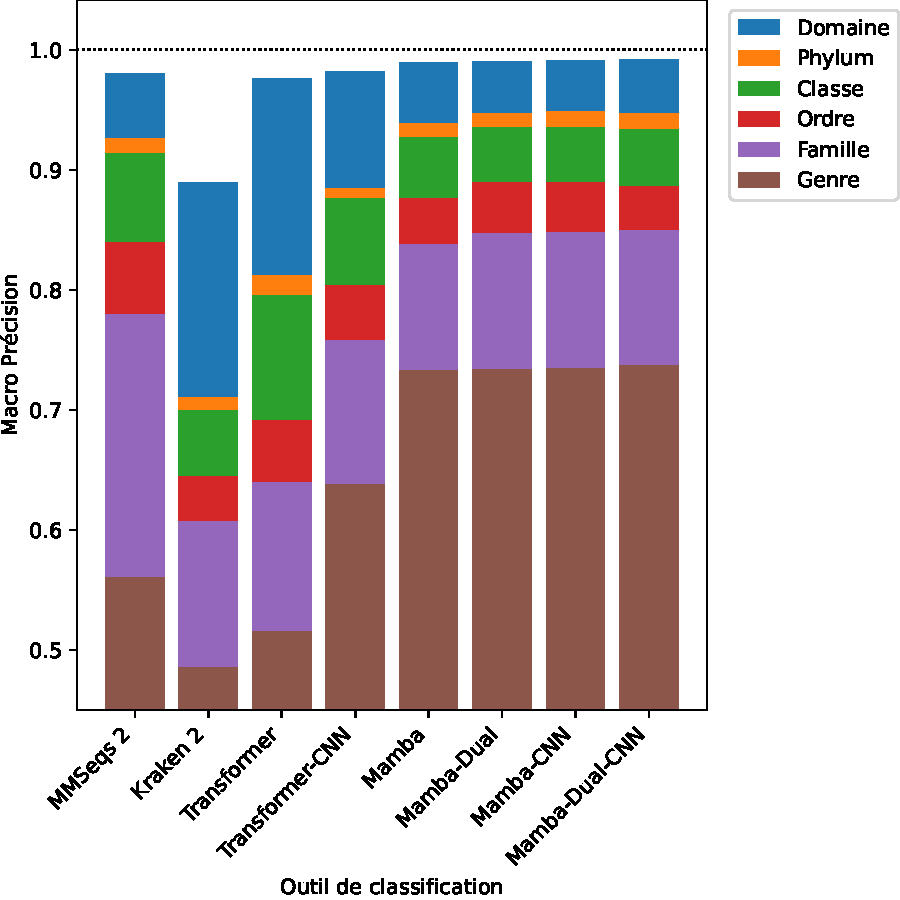
\includegraphics[width=\linewidth]{figures/dataset_2_taxa_Precision.pdf}
  \centering
  \caption{Précision macro à 6 niveaux taxonomiques pour le jeu de données 2}
    \label{fig:2_n_p}
\end{figure}

\begin{figure}[hbt!]
  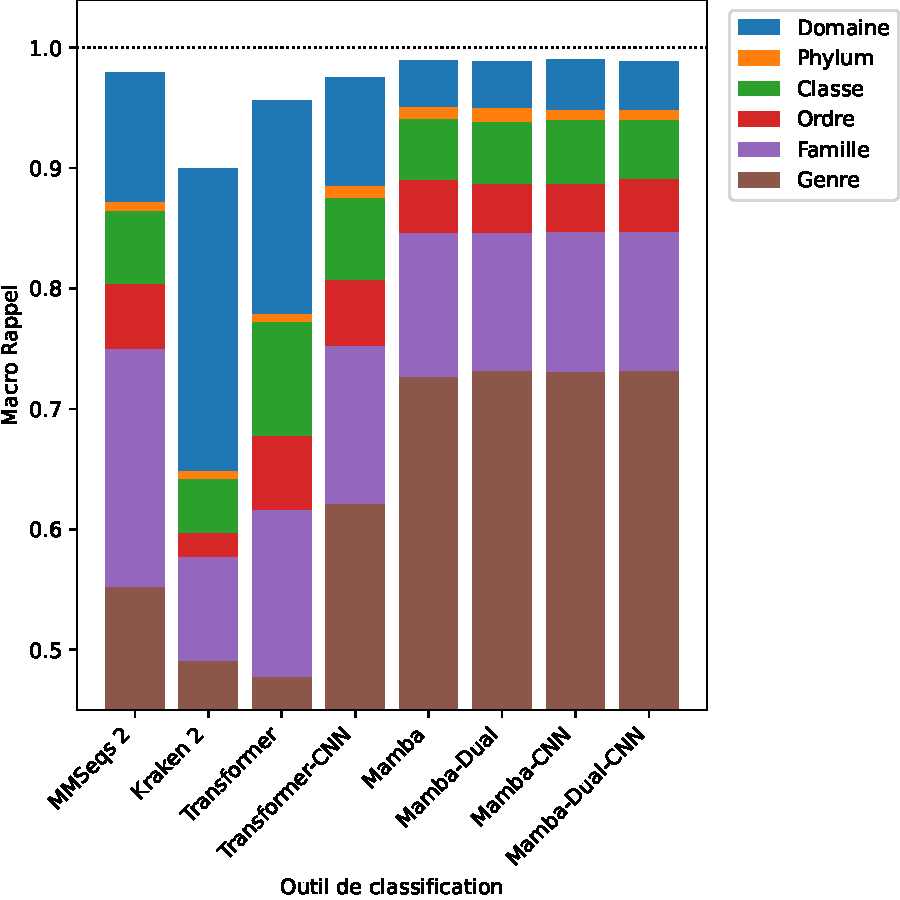
\includegraphics[width=\linewidth]{figures/dataset_2_taxa_Rappel.pdf}
  \centering
  \caption{Rappel macro à 6 niveaux taxonomiques pour le jeu de données 2}
    \label{fig:2_n_r}
\end{figure}

\begin{figure}[hbt!]
  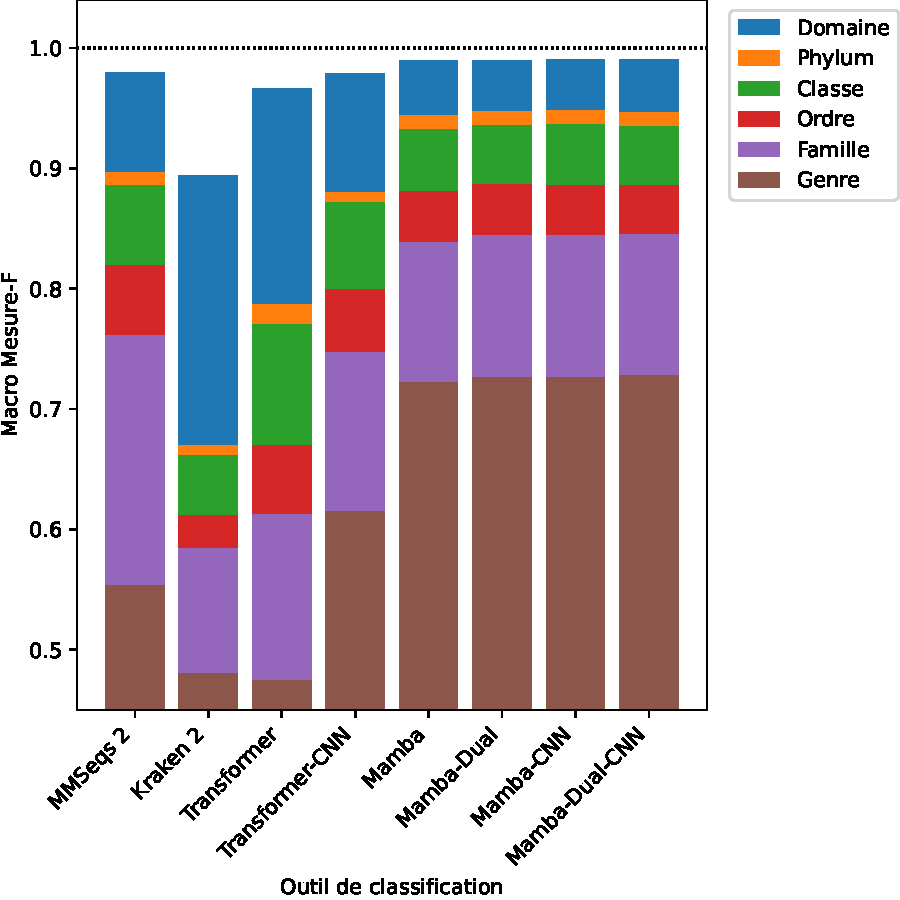
\includegraphics[width=\linewidth]{figures/dataset_2_taxa_Mesure-F.pdf}
  \centering
  \caption{Mesure-F macro à 6 niveaux taxonomiques pour le jeu de données 2}
    \label{fig:2_n_f}
\end{figure}


% Violon
Les figures \ref{fig:2_v_p}, \ref{fig:2_v_r} et \ref{fig:2_v_f} montrent les performances des
modèles à différents niveaux taxonomiques. Les barres horizontales indiquent les médianes.

\begin{figure}[hbt!]
  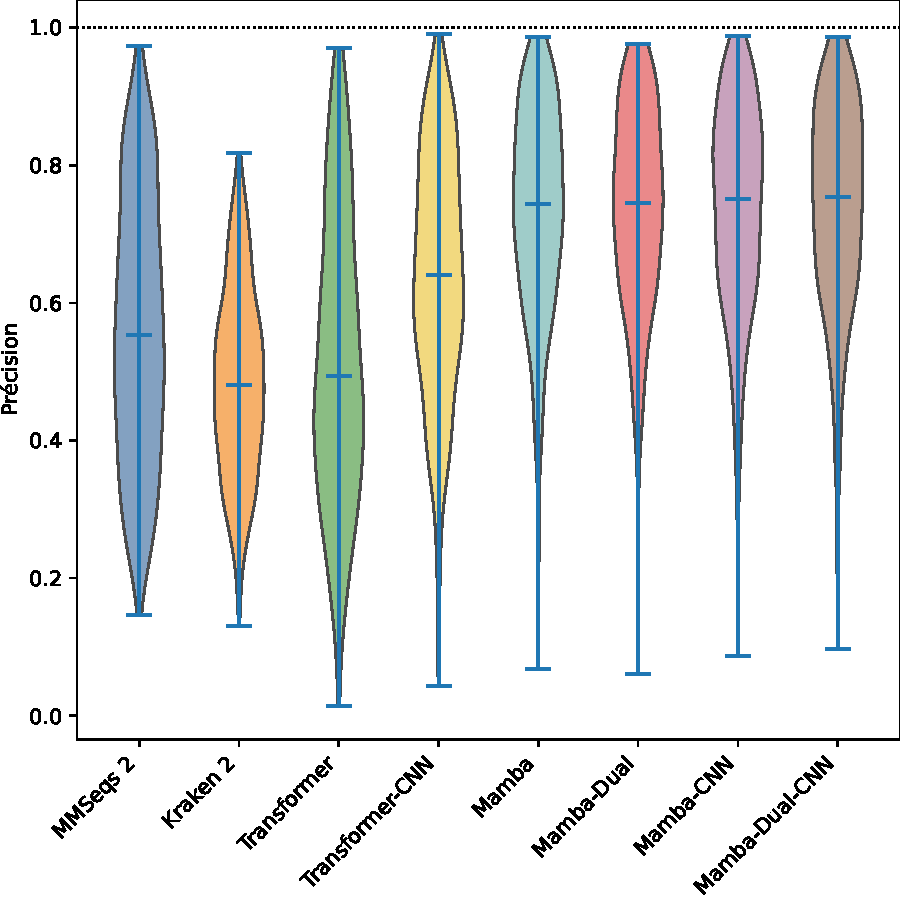
\includegraphics[width=\linewidth]{figures/dataset_2_violinplot_precision.pdf}
  \centering
  \caption{Diagramme violon de la précision macro pour le jeux de données 2}
  \label{fig:2_v_p}
\end{figure}

\begin{figure}[hbt!]
  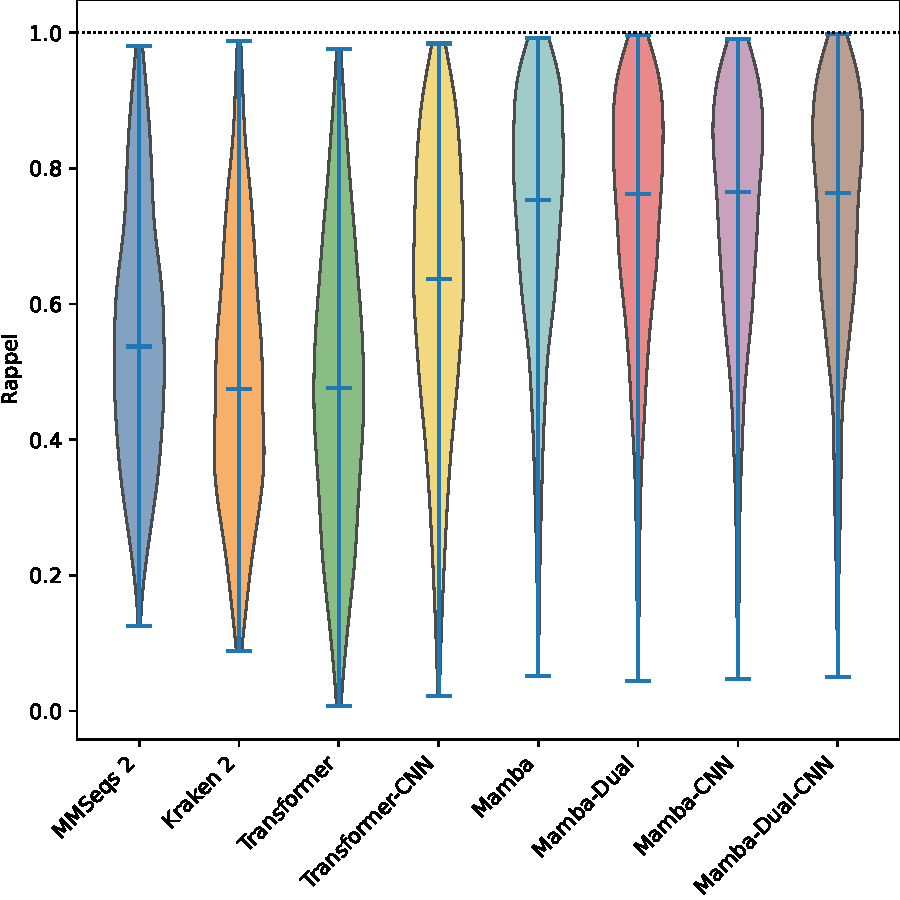
\includegraphics[width=\linewidth]{figures/dataset_2_violinplot_recall.pdf}
  \centering
  \caption{Diagramme violon du rappel macro pour le jeux de données 2}
  \label{fig:2_v_r}
\end{figure}

\begin{figure}[hbt!]
  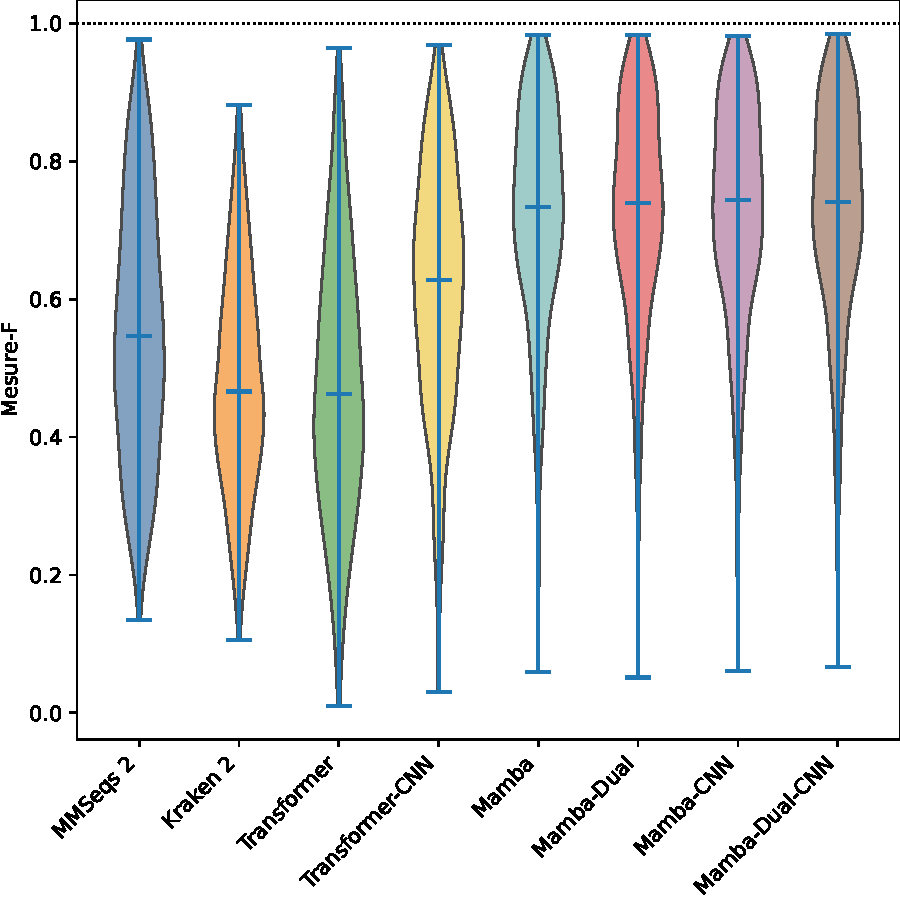
\includegraphics[width=\linewidth]{figures/dataset_2_violinplot_f1.pdf}
  \centering
  \caption{Diagramme violon de la mesure-F macro pour le jeux de données 2}
  \label{fig:2_v_f}
\end{figure}




% index
\printnoidxglossary[toctitle=INDEX,title=INDEX]

\bibliographystyle{apalike-uqam}
\bibliography{references}
\end{document}
